\begin{appendices}

\chapter{}

\enlargethispage{\baselineskip}
%\enlargethispage{\baselineskip}
\section{Extensión de la Herramienta IDA}

La herramienta Identifyer Analizer (IDA) tiene una característica extra, puede recibir como parámetro de entrada la ruta\footnote[1]{La ruta del archivo en un sistema de archivos de un sistema operativo determinado.} de un archivo XML (Extensible Markup Language). Este archivo debe contener información asociada a ids, literales y comentarios (propia de una aplicación JAVA); esta información es similar a la que es capturada por el Analizador Sintáctico que IDA posee (Módulo de Extracción de Datos - Ver Capítulo 4).
La herramienta IDA se encarga de leer la información provista por el archivo xml y ejecutar directamente los algoritmos de análisis de ids que tiene implementada. Por último, los resultados de la ejecución se escriben en otro archivo XML que será creado en la misma ruta que el archivo leído como entrada \mbox{(Ver Figura \ref{arq1}).}

La ventaja de que IDA soporte interacción con archivos XML, permite un intercambio de datos estándar con otras aplicaciones, lo que conlleva a tener compatibilidad para compartir información. De esta forma, IDA puede formar parte de un proceso de análisis más extenso que involucre otras herramientas asociadas a la comprensión de sistemas.

\vspace{-0.5em}

\begin{figure}[h!] %[h] para here [b] para bottom [t] para top
\centerline{%queda centrada mejor la imagen
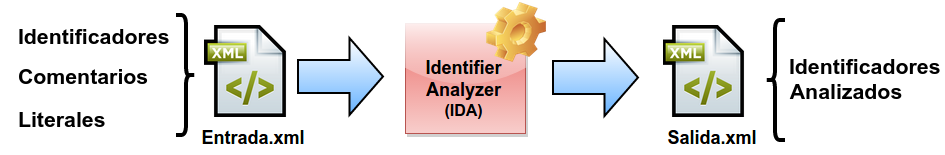
\includegraphics[scale= 0.57]{./ape/ape_01.png}
}
\caption{Arquitectura de la Extensión de IDA}
\label{arq1}
\end{figure}


\newpage

Para ingresar en IDA un archivo XML, simplemente se realiza a través del archivo JAR\footnote[1]{JAVA Archive.} (correspondiente a la herramienta), ejecutando la siguiente orden en la línea de comandos del sistema operativo\footnote[2]{Se recomienda utilizar los sistemas operativos Windows o UNIX con \textit{java runtime enviroment} instalado}:


\begin{lstlisting}[style=BashInputStyle]
  java -jar IDA.java <argumento>
\end{lstlisting}


En $<$\textsf{argumento}$>$ se coloca la ruta donde se encuentra ubicado el archivo XML a procesar (un ejemplo en linux es \textsf{/home/entrada.xml}\footnote[3]{No es necesario que se llame entrada, pero si que tenga extensión xml.}). Este argumento no es obligatorio, y en caso de no pasarlo, se ejecuta la interfaz normal de IDA que fue descripta en el capítulo 4.
La herramienta IDA procesa el archivo XML ingresado ejecutando los algoritmos de análisis de ids que tiene implementados (Greedy, Samurai y Expansión Básica).
A continuación, se describe como debe estar estructurado el archivo XML de entrada.

\noindent \textbf{\\Archivo XML de Entrada\\} 

El archivo xml que se ingresa, el comienzo debe marcarse con \mbox{$<$\textsf{entrada}$>$} y el fin con \mbox{$<$/\textsf{entrada}$>$} (Ver Figura \ref{xml1}), en su interior puede contener las siguientes listas de elementos:

\begin{description}
\itemsep0em%reduce espacio
\item[Lista de Identificadores:] Lista de ids que van a ser analizados, se enmarca con \mbox{$<$\textsf{lista\_ids}$>$} y \mbox{$<$/\textsf{lista\_ids}$>$}; cada elemento de esta lista se indica con $<$\textsf{id}$>$ y $<$/\textsf{id}$>$; dentro de cada uno de estos elementos se coloca: el nombre del id con \mbox{$<$\textsf{nombre}$>$\textbf{nmId}$<$/\textsf{nombre}$>$}, y el número de línea con \mbox{$<$\textsf{linea}$>$\textbf{45}$<$/\textsf{linea}$>$} (Ver Figura \ref{xml1}).

\item[Lista de Frases:] Listado de frases (asociadas a comentarios y literales) el inicio y fin de esta lista se indica con \mbox{$<$\textsf{lista\_frases}$>$} y \mbox{$<$/\textsf{lista\_frases}$>$};
cada elemento de esta lista se enmarca con $<$\textsf{frase}$>$ y $<$/\textsf{frase}$>$; dentro de cada uno de estos elementos de la lista se agrega: la frase correspondiente con \mbox{$<$\textsf{texto}$>$\textbf{File System}$<$/\textsf{texto}$>$}, y el número de línea con \mbox{$<$\textsf{linea}$>$\textbf{25}$<$/\textsf{linea}$>$} (Ver Figura \ref{xml1}).

\item[Lista de Clases:] Este listado se corresponde a las clases que posee el programa, se enmarca con \mbox{$<$\textsf{lista\_clases}$>$} y \mbox{$<$/\textsf{lista\_clases}$>$}; cada elemento de este listado se indica con $<$\textsf{clase}$>$ y $<$/\textsf{clase}$>$; en cada uno de estos elementos se agrega: el nombre del método  \mbox{$<$\textsf{nombre}$>$\textbf{Person}$<$/\textsf{nombre}$>$}, el número de línea donde comienza la clase \mbox{$<$\textsf{linea\_inicio}$>$\textbf{12}$<$/\textsf{linea\_inicio}$>$}, y la línea donde finaliza la clase \mbox{$<$\textsf{linea\_fin}$>$\textbf{38}$<$/\textsf{linea\_fin}$>$} (Ver Figura \ref{xml1}). 

\item[Lista de Métodos:] Similar al listado anterior pero para métodos, se enmarca con \mbox{$<$\textsf{lista\_metodos}$>$} y \mbox{$<$/\textsf{lista\_metodos}$>$}; cada elemento de este listado se indica con $<$\textsf{metodo}$>$ y $<$/\textsf{metodo}$>$; en cada uno de estos elementos se coloca: el nombre del método \mbox{$<$\textsf{metodo}$>$\textbf{getPerson}$<$/\textsf{metodo}$>$}, la línea donde comienza el método \mbox{$<$\textsf{linea\_inicio}$>$\textbf{20}$<$/\textsf{linea\_inicio}$>$}, y la línea donde finaliza la método \mbox{$<$\textsf{linea\_fin}$>$\textbf{25}$<$/\textsf{linea\_fin}$>$} (Ver Figura \ref{xml1}).

\end{description}

Es importante tener en cuenta, que el dato obligatorio en el archivo xml ingresado son los nombres de los ids, dado que es la principal fuente de información a analizar. Por otro lado, el resto de los datos: Métodos, Clases, Frases, números de líneas (de cualquier elemento), también son importantes, pero solo colaboran con el análisis de los ids y no son indispensables.
 
Luego de que IDA analiza los ids, el próximo paso es escribir los resultados de cada ejecución en un nuevo archivo XML de salida que se describe en la siguiente sección.


%\begin{description}
%\itemsep0em%reduce espacio
%\item[Lista de ids analizados:] Cada elemento de la lista posee, el nombre del id analizado, la correspondiente división Greedy, Samurai y las expansiones desde Greedy y Samurai.
%\end{description}


\newpage
\begin{figure}[h!] %[h] para here [b] para bottom [t] para top
\begin{lstlisting}[language=xml, frame=single]
<entrada>
	<lista_ids>
		<id>
		    <nombre>nmId</nombre>
		    <linea>10</linea>
		</id>    
		<id>	    	
		    <nombre>fs</nombre>
		    <linea>12</linea>
		</id>    	    	    
	</lista_ids>
	<lista_frases>
		<frase>
			<texto>name identifier</texto>
			<linea>9</linea>
		</frase>
		<frase>
			<texto>file system</texto>
			<linea>19</linea>
		</frase>
	</lista_frases>
	<lista_clases>
		<clase>
			<nombre>Person</nombre>
			<linea_inicio>7</linea_inicio>
			<linea_fin>30</linea_fin>
		</clase>
	</lista_clases>
	<lista_metodos>
		<metodo>
			<nombre>getPerson</nombre>
			<linea_inicio>11</linea_inicio>
			<linea_fin>19</linea_fin>
		</metodo>				
	</lista_metodos>	
</entrada>

\end{lstlisting}
\caption{Ejemplo de Archivo XML de entrada.}
\label{xml1}
\end{figure}

\newpage

\noindent \textbf{Archivo XML de Salida\\}

El archivo de salida contiene los ids analizados por las distintas técnicas y se crea en la misma ubicación que el archivo XML pasado por entrada (siguiendo con el ejemplo de la sección anterior se creará en \textsf{/home/salida.xml}\footnote[1]{Si ya existe un archivo con el nombre salida.xml, el mismo se sobrescribirá.}). Este archivo xml se le indica el inicio con \mbox{$<$\textsf{salida}$>$} y el fin con \mbox{$<$/\textsf{salida}$>$} (Ver Figura \ref{xml2}), en su interior posee la siguiente lista:

\begin{description}
\itemsep0em%reduce espacio
\item[Lista de Identificadores Analizados:] Es el listado de los ids incluyendo el análisis realizado en cada uno, $<$\textsf{lista\_analisis\_ids}$>$ señala el comienzo a la lista y $<$/\textsf{lista\_analisis\_ids}$>$ indica el fin; cada elemento de la lista se indica con $<$\textsf{id}$>$ y $<$/\textsf{id}$>$; dentro de cada elemento de la lista se encuentra: el nombre del id analizado enmarcado con \mbox{$<$\textsf{nombre}$>$\textbf{nmId}$<$/\textsf{nombre}$>$}, la división greedy del id se ubica entre \mbox{$<$\textsf{div\_greedy}$>$\textbf{nm-id}$<$/\textsf{div\_greedy}$>$}, la división samurai del id entre\\ \mbox{$<$\textsf{div\_samurai}$>$\textbf{nm-id}$<$/\textsf{div\_samurai}$>$}, la expansión desde greedy entre \mbox{$<$\textsf{exp\_greedy}$>$\textbf{name identifier}$<$/\textsf{exp\_greedy}$>$}, y la expansión desde samurai entre $<$\textsf{exp\_samurai}$>$\textbf{name identifier}$<$/\textsf{exp\_samurai}$>$ (Ver Figura \ref{xml2}).
\end{description}

\enlargethispage{\baselineskip}%agrega linea al final de la hoja.
\enlargethispage{\baselineskip}
\enlargethispage{\baselineskip}
\enlargethispage{\baselineskip}
\enlargethispage{\baselineskip}

\begin{figure}[h!]
\begin{lstlisting}[language=xml, frame=single]
<salida>
  <lista_analisis_ids>
    <id>
      <nombre>nmId</nombre>
      <div_greedy>nm-id</div_greedy>
      <div_samurai>nm-id</div_samurai>
      <exp_greedy>name identifier</exp_greedy>
      <exp_samurai>name identifier</exp_samurai>
    </id> 
    <id>
      <nombre>fs</nombre>
      <div_greedy>fs</div_greedy>
      <div_samurai>fs</div_samurai>
      <exp_greedy>file system</exp_greedy>
      <exp_samurai>file system</exp_samurai>
    </id>         
  </lista_analisis_ids>
</salida>
\end{lstlisting}
\caption{Ejemplo de Archivo XML de salida.}
\label{xml2}
\end{figure}

\end{appendices}


